\documentclass[12pt, a4paper]{article}

\usepackage[utf8]{inputenc}
\usepackage[T1]{fontenc}
\usepackage[russian]{babel}
\usepackage[oglav,spisok,boldsect, figwhole]{./style/fn2kursstyle1}
\graphicspath{{./style/}{./figures/}}
%\usepackage{float}%"Плавающие" картинки
\usepackage{multirow}
\usepackage{subcaption}
\usepackage{float}%"Плавающие" картинки
%Римские цифры
\newcommand{\RomanNumeralCaps}[1]
{\MakeUppercase{\romannumeral #1}}

\usepackage{enumitem} 
\usepackage{amsmath}
\usepackage{comment}
\usepackage{makecell}

%Параметры титульника
\title{Методы численного решения\\ интегральных уравнений}
\group{ФН2-62Б}
\author{З.И.~Абрамов, Г.А.~Швецов}
\supervisor{С.А.~Конев}
\date{2023}
\begin{document}
	\newcommand{\pl}{\partial}
	\maketitle
	
	\tableofcontents
	
	\newpage
	
	\section{Контрольные вопросы}
	\begin{enumerate}
		\item \textit{При выполнении каких условий интегральное уравнение Фредгольма 2-го рода имеет решение? В каком случае решение является единственным?}
		\smallskip
		
		\textbf{Интегральное уравнение Фредгольма 2-го рода}
		\[
		u(x)-\lambda\int\limits_a^bK(x,\xi)u(\xi)d\xi=f(x),\quad x\in[a,b].
		\]
		Ядро $K$ этого уравнения задано в квадрате $[a,b]\times[a,b]$.
		
		Существование решения уравнения Фредгольма 2-го рода и его единственность зависят от параметра  $\lambda$.
		\begin{enumerate}	
			\item Если $\lambda\ne\lambda_i\;(\lambda_i$ -- собственное число), то уравнение имеет единственное решение.
			\item $\lambda=\lambda_i$, т.е. параметр совпадает с одним из собственных значений, то при некоторых правых частях решение вообще не существует, а при других -- существует и неединственно.
			\item Множество собственных значений уравнения Вольтерры 2-го рода пусто. Поэтому неоднородное уравнение имеет решение, и притом единстенное.
		\end{enumerate}
		
		\textbf{Теорема.} Если $\lambda$ не является характеристическим числом, то интегральное уравнение Фредгольма 2-го рода имеет, и притом единственное, решение для любой непрерывной функции $f(x)$.
		\item \textit{Можно ли привести матрицу СЛАУ, получающуюся при использовании метода квадратур, к симметричному виду в случае, если ядро интегрального уравнения является симметричным, т.е. $K(x,\,s)=K(s,\,x)$?}
		\smallskip
		
		Да, можно. При использовании метода квадратур, получаем СЛАУ в следующем виде
		\[
		y_i-\lambda\sum_{k=0}^Na_k^N
		K(x_i,s_k)y_k=f_i, \qquad i=0,\dots,N.			
		\]
		Так как ядро интегрального уравнения симметричное, то $K(x_i,s_k)=K(s_k,x_i).$ Если умножить каждое $i$-е уравнение системы на $a_i^N$
		\[
		a_i^Ny_i-\lambda\sum_{k=0}^Na_i^Na_k^N
		K(x_i,s_k)y_k=a_i^Nf_i, \qquad i=0,\dots,N,			
		\]
		то получаем систему с симметричной матрицей.
		\item \textit{Предложите способ контроля точности результата вычислений при использовании метода квадратур.}
		\smallskip
		
		Последовательно дробим шаг сетки $h$ и сравниваем величину нормы разности вычисленного значения интеграла с требуемой точностью.
		\item \textit{Оцените возможность и эффективность применения методов квадратур, простой итерации и замены ядра при решении интегральных уравнений Вольтерры 2-го рода.}
		\smallskip
		\begin{enumerate}
			\item Итерационные методы, в частности метод простой итерации, также применимы к решению интегрального уравнения Фредгольма 2-го рода. Достаточным условием сходимости метода простой итерации в норме $\|.\|_C$ является выполнение условия
			\[
			|\lambda|\cdot \max\limits_{a\le x\le b}\int\limits_a^b|K(x,s)|ds\le1.
			\]
			Недостатком метода простой итерации является необходимость приближенного вычисления большого количества интегралов, что может приводить к значительным затратам машинного времени.
			\item Возможно применение метода квадратур. Получаем СЛАУ
			\[
			y_i-\lambda\sum_{k=0}^Na_k^N
			K(x_i,s_k)y_k=f_i			\]
			с треугольной матрицей, которая решается за один ход метода Гаусса. При этом решение существует и единственно для любого $\lambda$.
			\item Ядро интегрального уравнения Фредгольма называется вырожденным, если оно представимо в виде
			\[
			K(x,s)=\sum_{i=1}^m\phi_i(x)\psi_i(s),
			\]
			где $\phi_i(x),\,i=1,\dots,m$ -- система линейно независимых функций. А вот ядро уравнения Вольтерры вырожденным не бывает. Следовательно, метод замены ядра вырожденным для уравнения Вольтерры 2-го рода не применим.
		\end{enumerate}
		\item \textit{Что называют резольвентой ядра интегрального уравнения?}
		\smallskip
		
		Рассмотрим интегральное уравнение
		\begin{equation}
			f(s)+\lambda\int\limits_a^bK(s,t)\varphi(t)dt=\varphi(s).
			\label{inteq}
		\end{equation}
		\textbf{Резольвентой интегрального уравнения}, или его \textbf{разрешающим ядром} называется такая функция $R(s,t,\lambda)$, что решение уравнения \ref{inteq} представляется в виде
		\[
		u^*(s)=f(s)+\lambda\int\limits_a^bR(s,t,\lambda)f(t)dt.
		\]
		При этом $\lambda$ не должна быть собственным числом уравнения (\ref{inteq})
		\item \textit{Почему замену ядра интегрального уравнения вырожденным предпочтительнее осуществлять путем разложения по многочленам Чебышева, а не по формуле Тейлора?}
		\smallskip
		
		Полином Чебышева наилучшим образом аппроксимирует функцию на всем исследуемом отрезке. Формула же Тейлора записывается в окрестности точки, соответственно, чем дальше находится точка, в которой вычисляется приближенное значение функции, тем больше погрешность аппроксимации. Соответственно, замену ядра интегрального уравнения вырожденным предпочтительнее осуществлять путем разложения по многочленам Чебышева.
		\item \textit{Какие вы можете предложить методы решения переопределенной системы (5.13), (5.17) помимо введения дополнительно переменной $R$?}
		\smallskip
		
		Для решения переопределенной СЛАУ применим метод наименьших квадратов или метод вращений.
		
	\end{enumerate}
	
	\newpage
	\section{Дополнительные задачи}
	
	\begin{enumerate}
		\item \textit{Метод квадратур. Какие квадратуры Вы использовали в данной лабораторной работе? Какую точность они имеют (порядок, ведущий член погрешности)? Подтвердите расчетами, что такая же точность достигается в Вашей реализации квадратурных формул.}
		\smallskip
		
		В лабораторной работе была использована квадратурная формула трапеций:
		\[
		\int_{x_i}^{x_{i+1}} f(x) dx \approx \frac{f(x_i)+f(x_{i+1})}2 h, \qquad h = x_{i+1} - x_i,
		\]
		которая имеет оценку локальной погрешности
		\[
		|\psi_{h, i}| \le \frac1{12} M_2 h^3.
		\]
		Отсюда получаем оценку погрешности квадратурной формулы трапеции
		\[
		|\psi_h| \le \frac1{12} M_2 h^3 n = \frac1{12} M_2 h^3 \frac{b-a}{h} = \frac1{12} M_2 (b-a) h^2 = O(h^2).
		\]
		
		% TODO
		
		\item \textit{Критерий останова. Какой критерий останова использовался для метода простой итерации? Вычислите априорную оценку погрешности (приведена в методическом пособии), содержащую множитель}
		\[
		q = |\lambda| \max_{a \le x \le b} \int_a^b |K(x, s)| ds.
		\]
		\textit{Проверьте, действительно ли достигаемая точность меньше оцениваемой.}
		\smallskip
		
		Для метода простой итерации в качестве критерия останова было выбрано условие, что норма разности между последними приближениями меньше некоторого заданного $\varepsilon$:
		\[
		\|u^{(k+1)} - u^{(k)}\| < \varepsilon.
		\]
		
		% 8 номер из скинутой методички
		В качестве тестового примера возьмем уравнение
		\[
		u(x) - \frac1{2\pi} \int_0^\pi s \sin x\,u(s) ds = \cos x, \qquad x, s \in [0,\pi],
		\]
		точное решение которого имеет вид $u(x) = \cos x - \sfrac2\pi \sin x$.
		
		Для этого примера
		\[
		q = \left|\frac1{2\pi}\right| \max_{0 \le x \le \pi} \int_0^\pi |s \sin x| ds = \frac1{2\pi} \cdot \frac12 \pi^2 \max_{0 \le x \le \pi} \sin x = \frac\pi4 \approx 0.785398 < 1.
		\]
		
		Было взято 50 узлов.
		
		Для методов типа простой итерации существуют следующие оценки:
		\[
		\|u^{(k)} - u_*\| \le q^k \|u^{(0)} - u_*\|, \qquad \|u^{(k)} - u_*\| \le \frac{q^k}{1-q} \|u^{(1)} - u^{(0)}\|,
		\]
		где $u_*$ --- точное решение задачи, $k$ --- номер итерации. Будем использовать первую оценку. В качестве начального приближения примем правую часть уравнения $\cos(x)$. Тогда
		\[
		\|u^{(0)} - u_*\| = \left\|\frac2\pi \sin x\right\| = \frac2\pi.
		\]
		
		\begin{table}[H]
			\caption{Погрешность метода простой итерации}
			\centering
			\begin{tabular}{|c|l|l|}
				\hline
				Число итераций & Достигнутая точность & Теоретическая погрешность \\ \hline
				1        & 0.318205             & 0.5                       \\ \hline
				2        & 0.15905              & 0.392699                  \\ \hline
				3        & 0.0794989            & 0.308425                  \\ \hline
				4        & 0.0397364            & 0.242237                  \\ \hline
				5        & 0.0198616            & 0.190252                  \\ \hline
				6        & 0.00992754           & 0.149424                  \\ \hline
				7        & 0.00496212           & 0.117357                  \\ \hline
				8        & 0.00248023           & 0.092172                  \\ \hline
				9        & 0.00123969           & 0.0723917                 \\ \hline
				10       & 0.000619629          & 0.0568563                 \\ \hline
				11       & 0.000309699          & 0.0446549                 \\ \hline
				12       & 0.000154785          & 0.0350719                 \\ \hline
			\end{tabular}
		\end{table}
		
		В данном примере погрешность за одну итерацию уменьшается примерно в 2 раза.
		
		\item \textit{Замена ядра вырожденным. Как меняется погрешность решения с увеличением числа слагаемых в разложении ядра по формуле?}
		
		Для вычисления погрешности возьмем следующее интегральное уравнения:
		\[
		u(x)-4\int_0^1 x^2 e^{x^2 s^4} u(s) ds = x^3 - (e^{x^2}-1), \qquad s, t \in [0, 1],
		\]
		которое имеет  точное решение $u(x) = x^3$.
		
		Разложим ядро:
		\[
		K(x, s) = x^2 e^{x^2 s^4} = x^2 + \sum_{k=1}^\infty \frac{s^{4k}}{k!} x^{2(k+1)}.
		\]
		
		Число узлов: $N = 200$.
		
		\begin{table}[H]
			\caption{Погрешность при замене ядра вырожденным}
			\centering
			\begin{tabular}{|c|l|}
				\hline
				Число слагаемых & Достигнутая точность \\ \hline
				1        &         0.838659         \\ \hline
				2        &         0.100678         \\ \hline
				3        &         0.0199564         \\ \hline
				4        &         0.00348168         \\ \hline
				5        &         0.00059282         \\ \hline
				6        &         0.000181023         \\ \hline
				7        &         0.00010464         \\ \hline
				8        &         9.356e-05         \\ \hline
				9        &         9.31759e-05         \\ \hline
				10        &         9.31655e-05         \\ \hline
				11        &         9.31646e-05         \\ \hline
				12        &         9.31645e-05         \\ \hline
			\end{tabular}
		\end{table}
		
		\item \textit{Сингулярные уравнения. Установить расчетным путем наименьшее количество точек разбиения окружности, необходимое для получения точного решения сингулярного интегрального уравнения. Какое количество узлов потребовалось для передачи качественного характера решения?}
		
		В качестве исследуемого примера возьмем тест 2 из методического пособия с правой частью вида
		\[
		f(\vec{r}) = \sin(7\phi).
		\]
		
		Тогда точное решение имеет следующий вид:
		\[
		\gamma(\vec{r}) = -2 \cos(7\phi).
		\]
		
		Ниже приведена таблица, отражающая зависимость абсолютной ошибки в узлах от количества узлов N.
		
		\begin{table}[H]
			\caption{Абсолютная ошибка в зависимости от количества узлов}
			\centering
			\begin{tabular}{|c|l|}
				\hline
				Число узлов & Абсолютная ошибка \\ \hline
				4      & 4                 \\ \hline
				5      & 4                 \\ \hline
				6      & 4                 \\ \hline
				7      & 3                 \\ \hline
				8      & 3.9968e-15        \\ \hline
				9      & 4.44089e-15       \\ \hline
				10      & 7.54952e-15       \\ \hline
				11      & 6.66134e-15       \\ \hline
				12      & 7.32747e-15       \\ \hline
			\end{tabular}
		\end{table}
		
		Таким образом, наименьшее количество точек разбиения окружности, необходимое для получения точного решения сингулярного интегрального уравнения, равно 8. Однако при N = 12 картина выглядит следующим образом:
		\begin{figure}[H]
			\centering
			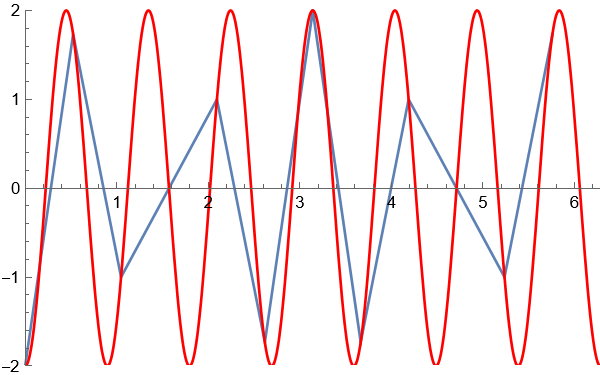
\includegraphics[width=0.7\linewidth]{bad.png}
		\end{figure}
		
		Для передачи качественного характера решения требуется примерно 30 узлов:
		\begin{figure}[H]
			\centering
			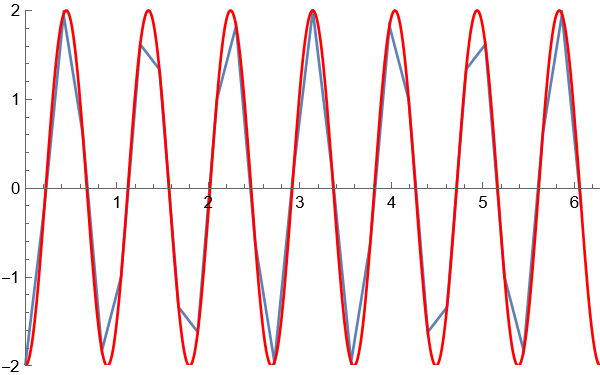
\includegraphics[width=0.7\linewidth]{good.png}
		\end{figure}
		
		\item \textit{Регуляризация. Для решения сингулярного интегрального уравнения в методическом пособии предлагается вводить дополнительную неизвестную R. Постройте таблицу, содержащую зависимость величины R от числа узлов сетки.}
		
		В качестве исследуемого примера возьмем тест 2 из методического пособия с правой частью вида
		\[
		f(\vec{r}) = \sin(\phi).
		\]
		
		Тогда точное решение имеет следующий вид:
		\[
		\gamma(\vec{r}) = -2 \cos(\phi).
		\]
		
		\begin{table}[H]
			\caption{Значение R при разных количествах узлов}
			\centering
			\begin{tabular}{|c|l|}
				\hline
				Число узлов & Значение R              \\ \hline
				10      & -3.21965e-16            \\ \hline
				20      & \hphantom{-}9.71445e-17 \\ \hline
				30      & -1.25918e-15            \\ \hline
				40      & \hphantom{-}6.21725e-16 \\ \hline
				50      & -3.59712e-16            \\ \hline
				60      & -2.9791e-16             \\ \hline
				70      & -3.17207e-18            \\ \hline
				80      & -8.24341e-16            \\ \hline
				90      & \hphantom{-}1.38161e-16 \\ \hline
				100     & \hphantom{-}1.9984e-16  \\ \hline
			\end{tabular}
		\end{table}
		
		% TODO
		
	\end{enumerate}
	
	\newpage
	\section{Результаты}
	\[
	u(x)-\int\limits_a^b\frac12(1-x\cos(xs))u(s)\,ds=f(x),\quad x\in[a,b],
	\]
	\begin{enumerate}
	\item $ f(x)=\sfrac12(1+\sin x).$
	\begin{enumerate}
			\centering
		\item $x\in[0,1]$
		\begin{figure}[H]
			\centering
			\begin{subfigure}[b]{0.45\textwidth}
				\centering
				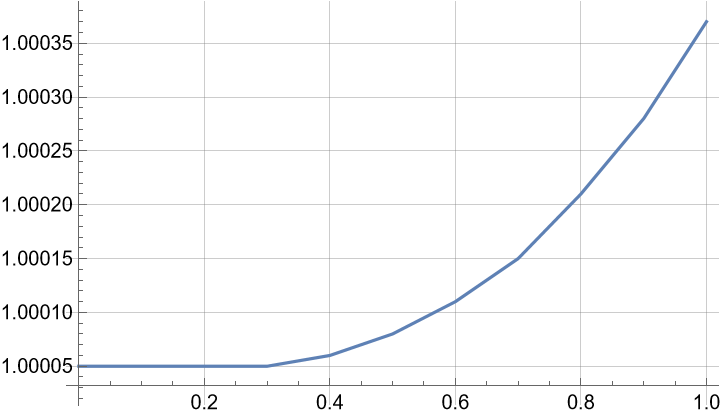
\includegraphics[width=\textwidth]{task1_1_1_simple}
				\caption{Метод простой итерации}
			\end{subfigure}
			\hfill
			\begin{subfigure}[b]{0.45\textwidth}
				\centering
				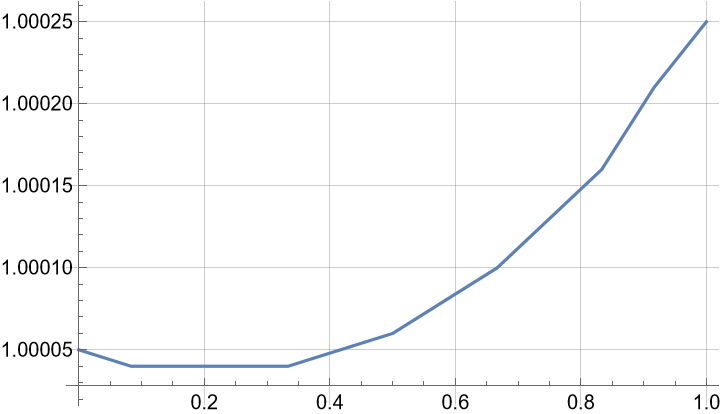
\includegraphics[width=\textwidth]{task1_1_1_quadro}
				\caption{Метод квадратур}
			\end{subfigure}
		\end{figure}
		\item $x\in[0.1,1]$
	\begin{figure}[H]
		\centering
		\begin{subfigure}[b]{0.45\textwidth}
			\centering
			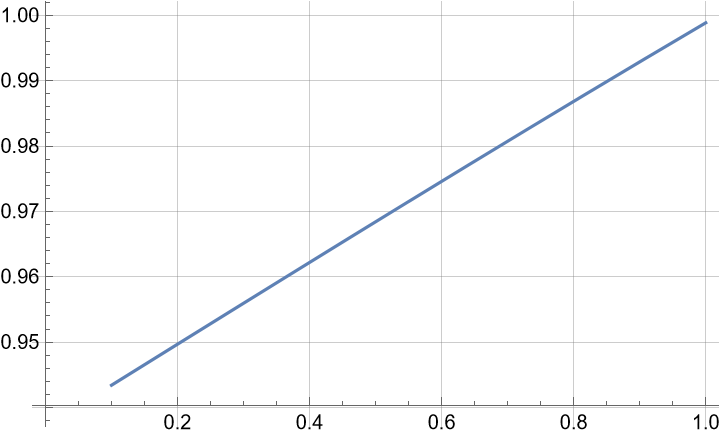
\includegraphics[width=\textwidth]{task1_1_2_simple}
			\caption{Метод простой итерации}
		\end{subfigure}
		\hfill
		\begin{subfigure}[b]{0.45\textwidth}
			\centering
			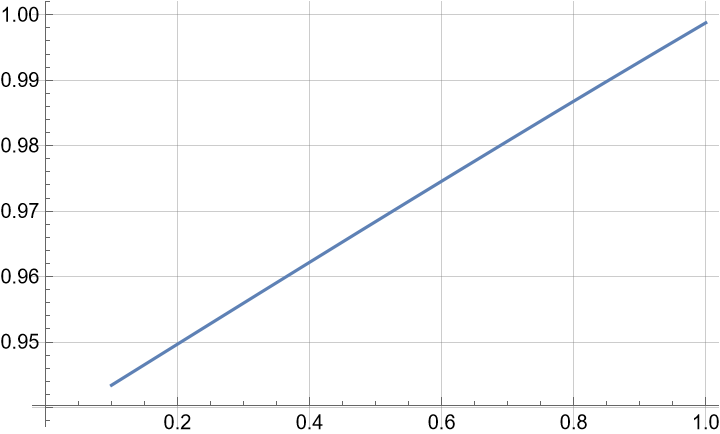
\includegraphics[width=\textwidth]{task1_1_2_quadro}
			\caption{Метод квадратур}
		\end{subfigure}
	\end{figure}
	\end{enumerate}
\newpage
\item $ f(x)=x^2+\sqrt x.$
\begin{enumerate}
	\centering
	\item $x\in[0,1]$
	\begin{figure}[H]
		\centering
		\begin{subfigure}[b]{0.45\textwidth}
			\centering
			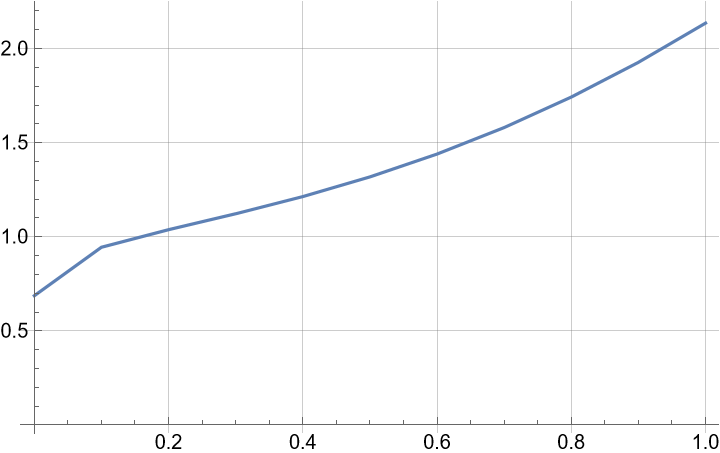
\includegraphics[width=\textwidth]{task1_2_1_simple}
			\caption{Метод простой итерации}
		\end{subfigure}
		\hfill
		\begin{subfigure}[b]{0.45\textwidth}
			\centering
			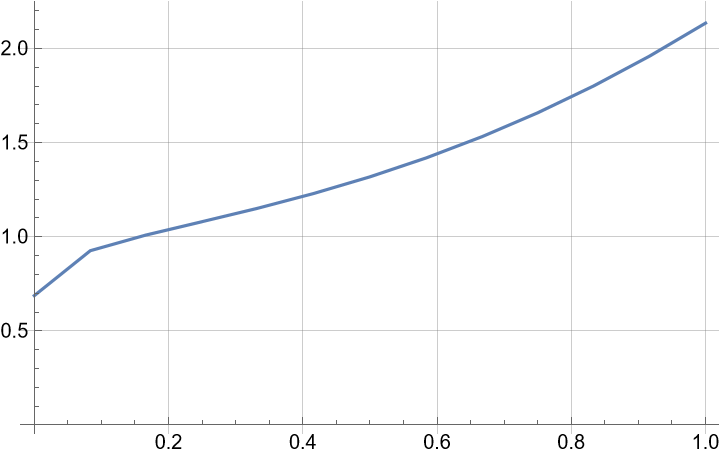
\includegraphics[width=\textwidth]{task1_2_1_quadro}
			\caption{Метод квадратур}
		\end{subfigure}
	\end{figure}
	\item $x\in[0.1,1]$
	\begin{figure}[H]
		\centering
		\begin{subfigure}[b]{0.45\textwidth}
			\centering
			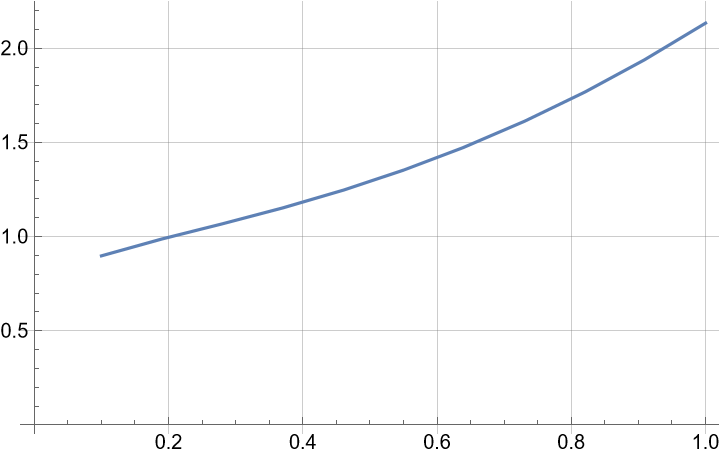
\includegraphics[width=\textwidth]{task1_2_2_simple}
			\caption{Метод простой итерации}
		\end{subfigure}
		\hfill
		\begin{subfigure}[b]{0.45\textwidth}
			\centering
			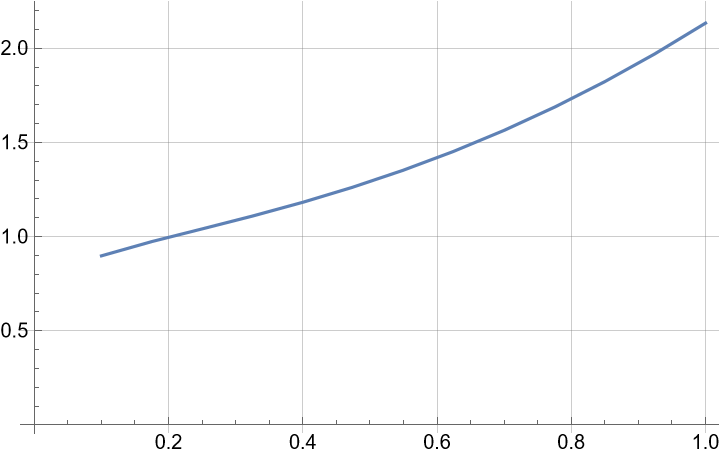
\includegraphics[width=\textwidth]{task1_2_2_quadro}
			\caption{Метод квадратур}
		\end{subfigure}
	\end{figure}
\end{enumerate}
	\end{enumerate}
	
	
	
	
	
	\newpage
	\begin{thebibliography}{1}
		\bibitem{galanin} \textit{Галанин М.П., Савенков Е.Б.} Методы численного анализа математических\\ моделей. М.: Изд-во МГТУ им. Н.Э. Баумана,	2010. 592 с.
		
		
	\end{thebibliography}
	
	
\end{document}
